\section{Eksperimenti 1. faze}
\subsection{Preliminarni testi}
\subsubsection{Optimizacija HOOF deskriptorjev}\label{sec:optimizacija-hoof}
Parameter $N_{HOOF}$ smo določili na podlagi rezultatov iz poglavja \ref{sec:rezultati-optimizacija-hoof}. Za evaluacijo smo uporabili učne vzorce hrbtne kamere preliminarnih laboratorijskih testov. Evaluirali smo samo za podatke energijske porabe $W$. Pridobljene značilke deskriptorjev smo normirali na intervalu $[-1,1]$ in jih uporabili za učenje regresijskega modela z metodo podpornih vektorjev $\epsilon$-SVR in jedrom RBF. Metode so podrobneje predstavljene v poglavju \ref{sec:matematicni-modeli}. Za določitev optimalnih parametrov, ki so predstavljeni v tabeli \ref{tab:nhoof-param}, smo uporabili optimizacijsko metodo mrežnega iskanja \cite{hsu2003practical}. Rezultate smo filtrirali še s Kalmanovim filtrom, ki je predstavljen v \ref{sec:kalmanov-filter}.

\begin{table}[htb]
	\centering
	\begin{tabular}{S[table-format=2.0] S[table-format=2.3] S[table-format=1.3] S[table-format=1.3] S[table-format=1.3]}
		\toprule
		\thead{$\mathbf{N_{HOOF}}$} & \thead{$\mathbf{C}$} & \thead{$\mathbf{\gamma}$} & \thead{$\mathbf{\epsilon}$} & \thead{MSE} \\ 
		\midrule
		30 & 8 & 0.707 & 0.812 & 7.903 \\
		60 & 8 & 0.354 & 0.379 & 7.320 \\
		120 & 11.314 & 0.177 & 0.536 & 6.998 \\
		160 & 11.314 & 0.125 & 0.616 & 6.832 \\
		\bottomrule
	\end{tabular}
	\caption[Optimalni parameteri RBF jedra modelov za določitev $N_{HOOF}$]{Optimalni parametri RBF jedra za modele z različnim številom stolpcev $N_{HOOF}$ v HOOF deskriptorju. Z njimi smo učili modele s katerimi smo preverjali optimalno število stolpcev v HOOF deskriptorju}
	\label{tab:nhoof-param}
\end{table}







\subsubsection{Optimizacija HAFA deskriptorjev}
Parameter $N_{HAFA}$ smo določili na podlagi rezultatov \ref{sec:rezultati-optimizacija-hafa}. Za evaluacijo smo uporabili enak eksperimentalni protokol kot za HOOF značilke v poglavju \ref{sec:hoof}, s to razliko, da smo značilke normirali na intervalu $[0, 1]$ in odstranili stolpec z amplitudami $0.5$. S tem smo odstranili šum, ki se je pojavil, ko ni bilo nobenega gibanja. Amplitudo šuma smo določili, kot maksimalno vrednost amplitude, ki še ni predstavljala gibanja. Optimalni parametri evaluacijske metode so predstavljeni v tabeli \ref{tab:nhafa-param}.


\begin{table}[!htb]
	\centering
	\begin{tabular}{S[table-format=2.0] S[table-format=2.3] S[table-format=1.3]  S[table-format=1.3] S[table-format=1.3]}
		\toprule
		\thead{$\mathbf{N_{HAFA}}$} & \thead{$\mathbf{C}$} & \thead{$\mathbf{\gamma}$} & \thead{$\mathbf{\epsilon}$} & \thead{MSE} \\ 
		\midrule
		30 & 8 & 5.657 & 0.616 & 4.329 \\
		60 & 8 & 5.657 & 0.616 & 4.327 \\
		120 & 8 & 5.657 & 0.616 & 4.327 \\
		160 & 8 & 5.657 & 0.616 & 4.327 \\
		\bottomrule
	\end{tabular}
	\caption[Optimalni parameteri RBF jedra modelov za določitev $N_{HAFA}$]{Optimalni parametri RBF jedra za modele z različnim številom stolpcev $N_{HAFA}$ v HAFA deskriptorju. Z njimi smo učili modele s katerimi smo preverjali optimalno število stolpcev v HAFA deskriptorju.}
	\label{tab:nhafa-param}
\end{table}






\subsubsection{Razširitev HOOF deskriptorja}\label{sec:razsiritev-hoof-rezultati}
HOOF deskriptorju smo pripeli HAFA deskriptor in tako dobili razširjeni deskriptor HOOF-HAFA, ki po evaluaciji iz poglavja \ref{sec:rezultati-razsiritev-hoof} v splošnem daje boljše rezultate.

Pri evaluaciji deskriptorjev HOOF in HOOF-HAFA smo uporabili učne vzorce hrbtne kamere terenskih testov. Evaluirali smo za podatke srčnega utripa $hr$. Srčni utrip smo za gradnjo modelov pretvorili v energijsko porabo $W$ po enačbi \eqref{eq:charlot}. Pridobljene značilke smo normirali na intervalu [0,1] in jih uporabili za učenje regresijskega modela z metodo podpornih vektorjev $\epsilon$-SVR in jedrom RBF. Za določitev optimalnih parametrov, ki so predstavljeni v tabeli \ref{tab:nhoof-param}, smo uporabili optimizacijsko metodo mrežnega iskanja \cite{hsu2003practical}. Rezultate smo filtrirali še s Gaussovim jedrom (predstavljen v \ref{sec:gaussov-filter}) velikosti $6$ in varianco $\sigma=16$. 

\begin{table}[htb]
	\centering
	\begin{tabular}{l S[table-format=2.3] S[table-format=1.3] S[table-format=1.3] S[table-format=1.3]}
		\toprule
		\textbf{Deskriptor} & \thead{$\mathbf{C}$} & \thead{$\mathbf{\gamma}$} & \thead{$\mathbf{\epsilon}$} & \thead{MSE} \\ 
		\midrule
		HOOF & 2.828 & 11.314 & 0.435 & 2.192 \\
		HOOF-HAFA & 5.657 & 2.828 & 0.154 & 1.781 \\
		\bottomrule
	\end{tabular}
	\caption[Optimalni parameteri RBF jedra modelov za izbiro deskriptorjev]{Optimalni parametri RBF jedra za modele z različnim deskriptorjem. Z modeloma smo preverjali razširitev HOOF deskriptorja v HOOF-HAFA deskriptor.}
	\label{tab:izbira-param}
\end{table}














\subsubsection{Testiranje sledilnikov za optični tok}\label{sec:testiranje-sledilnikov-za-opticni-tok}
Sledilnike smo testirali na sekvencah slik \textit{handball1} in \textit{handball2} podatkovne baze VOT2016 \cite{kristan2016visual}.Primer posnetkov je viden na sliki \ref{fig:testiranje-tracker-visual}. Sledila je še hitra vizualna ocena delovanja na kratkih izsekih video posnetka \cite{squashtv2014squash}. Primer posnetka je viden na sliki \ref{fig:testiranje-squash-1-kcf}.

\begin{figure}[!htbp]
	\centering
	
	\begin{subfigure}[t]{0.45\columnwidth}
		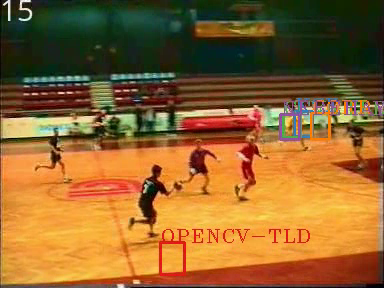
\includegraphics[width=\columnwidth]{./Slike/handball1-example.png}
		\caption{15. slika posnetka \textit{handball1}.}
		\label{fig:testiranje-handball1}
	\end{subfigure}
	~
	\begin{subfigure}[t]{0.45\columnwidth}
		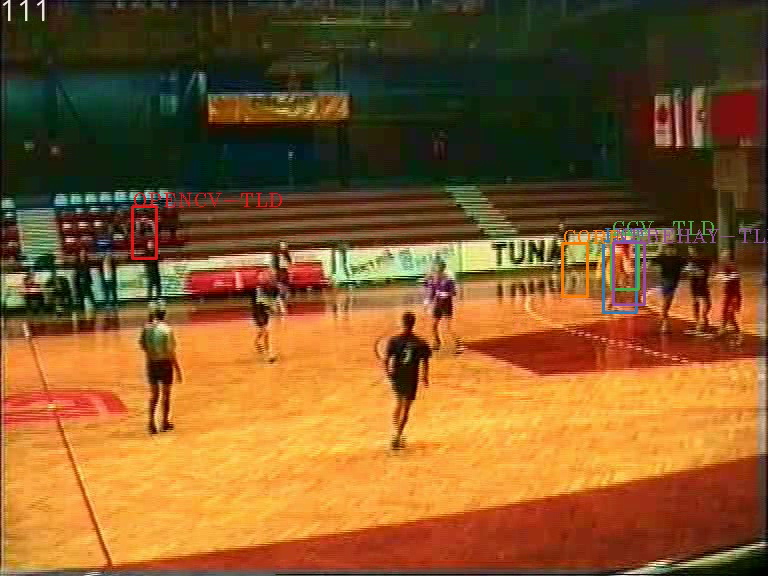
\includegraphics[width=\columnwidth]{./Slike/handball2-example.png}
		\caption{111. slika posnetka \textit{handball2}.}
		\label{fig:testiranje-handball2}
	\end{subfigure}  
	\caption[Primer delovanja sledilnikov za \textit{handball} posnetke]{Primer delovanja sledilnikov za \textit{handball} posnetke. Referenčni igralec, ki mu morajo slediti ima rumeno majico. }
	\label{fig:testiranje-tracker-visual}
\end{figure}



\begin{figure}[htbp]
	\centering
	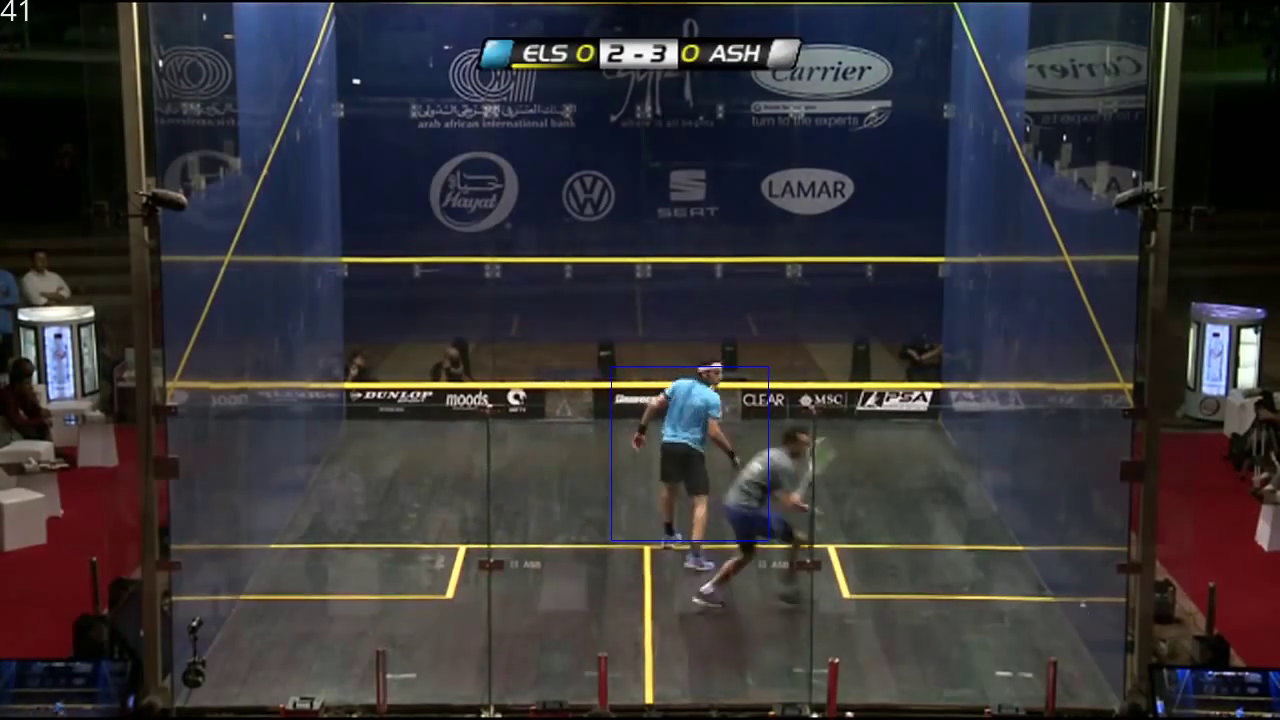
\includegraphics[width=0.6\columnwidth]{./Slike/squash-1-kcf-example.png}
	\caption[Uporaba squash posnetka za vizualno oceno delovanja sledilnikov]{Uporaba squash posnetka za vizualno oceno delovanja sledilnikov. Predstavljena je 41. slika posnetka \cite{squashtv2014squash}, kjer smo preizkušali KCF sledilnik. Sledili smo igralcu v svetlo modri majici. Modri okvir prikazuje področje, ki ga je sledilnik zaznal.}
	\label{fig:testiranje-squash-1-kcf}
\end{figure}



Pri testiranju sekvenc slik podatkovne baze VOT2016 smo poenostavili rotirajoča referenčna področja detekcij na nerotirajoča področja. Pri tem smo za zgornji levi kot $T_0(x,y)$ in spodnji desni kot $T_1(x,y)$ uporabili enačbo \eqref{eq:vot-bb}, kjer so $\left( x_i, y_i\right), \forall i=1,\ldots,4$ ogljišča rotirajočega referenčnega področja. 

\begin{equation}
\begin{aligned}
T_0(x,y) &= \left( \min_{i = 1,\ldots,4}\left\{x_i \right\}, 
\min_{i=1,\ldots,4}\{y_i \} \right) \\
T_1(x,y) &= \left( \max_{i = 1,\ldots,4}\left\{x_i \right\}, 
\max_{i=1,\ldots,4}\{y_i \} \right)
\end{aligned}
\label{eq:vot-bb}
\end{equation}

Ker je za naš sledilnik najbolj pomembno zanesljivo delovanje, smo izbrali mero prekrivanja področja.


Video posnetek \cite{squashtv2014squash} smo za potrebe vizualne ocene delovanja na squash posnetkih razdelili na več kratkih izsekov. Pri tem smo uporabili le hrbtne posnetke mirujoče kamere. 







\subsection{Laboratorijski eksperimenti tekalne steze}
Prve eksperimente smo izvedli v laboratoriju za fiziologijo na Fakulteti za šport. Merjenec je tekel na tekalni stezi ob prisotnosti operaterja---zdravnika, ki je določal intenziteto in čas trajanja obremenitve. Pri tem smo merili srčni utrip in enrgijsko porabo športnika (starost: 26 let, višina: \SI{177}{\cm}, teža: \SI{79.1}{\kg}, $VO_2max$: \SI{3705}{\ml\per\min}). Energijsko porabo smo merili z indirektno kalorimetrijo, in sicer s ``breath by breath'' Cosmed CPET Metabolic Cart \cite{beaver1973line}. Pri tem smo uporabili Hans Rudolph obrazno masko s predpisanim minimalnim VD (mrtvim prostorom).


\subsubsection{Pridobivanje podatkov}
Tekalno stezo smo snemali iz dveh različnih zornih kotov: hrbtni del in stranski del. Zaradi časovne neusklajenosti posnetkov smo jih sinhronizirali glede na začetno sliko meritev. Zaradi rahlo različne časovne frekvence na posameznih kamerah, se časovne neusklajenosti do potankosti nismo mogli znebiti. Ta se je akumulirala skozi čas. Primer hrbtnega in stranskega posnetka je prikazan na sliki \ref{fig:primer-posnetka-rgb}.

\begin{figure}[htb]
	\centering
	\begin{subfigure}{0.45\columnwidth}
		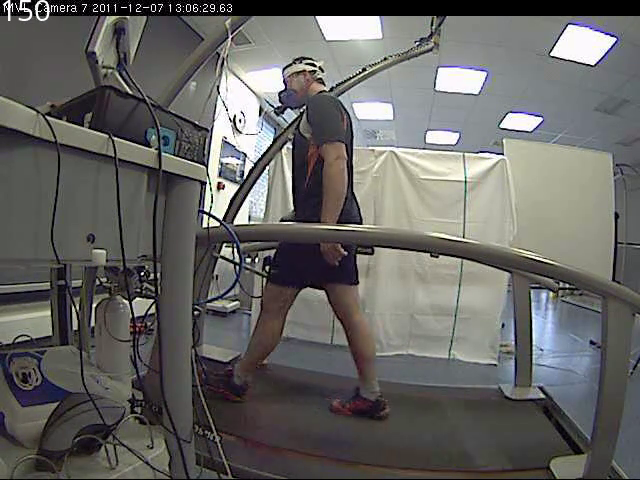
\includegraphics[width=\columnwidth]{./Slike/normal-sv-150.png}
		\caption{Stranska 150. slika.}
	\end{subfigure}
	~
	\begin{subfigure}{0.45\columnwidth}
		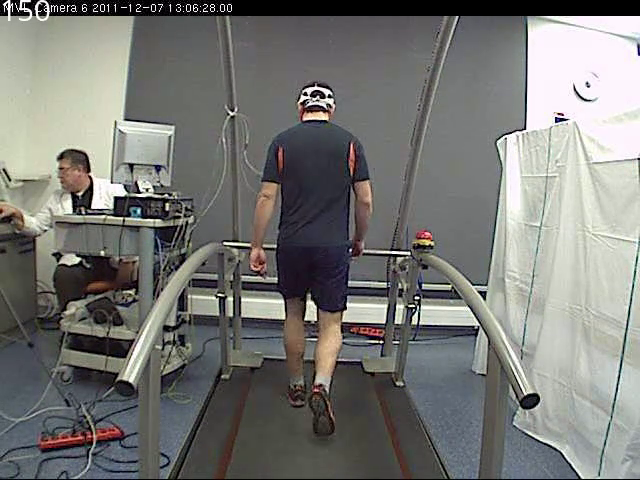
\includegraphics[width=\columnwidth]{./Slike/normal-bv-150.png}
		\caption{Hrbtna 150. slika.}
	\end{subfigure}
	\caption[Hrbtna in stranska 150. slika RGB posnetkov iz prve serije]{Hrbtna in stranska 150. slika RGB posnetkov iz prve serije. Kljub časovni sinhronizaciji med posnetkoma, se časovni neusklajenosti nismo mogli popolnoma izogniti. Časovni frekvenci kamer nista bili sinhronizirani.}
	\label{fig:primer-posnetka-rgb}
\end{figure}

Pridobili smo posnetke barvnih RGB slik in infrardeče IR posnetke hrbtnega dela. Primer IR posnetka za hrbntni pogled je prikazan na sliki \ref{fig:primer-posnetka-ir}.


\begin{figure}[htb]
	\centering
	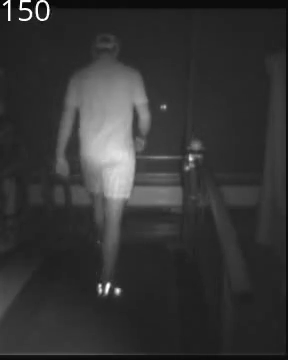
\includegraphics[width=0.25\columnwidth]{./Slike/normal-ir-150.png}
	\caption{Hrbtna 150. slika IR posnetka iz prve serije.}
	\label{fig:primer-posnetka-ir}
\end{figure}

Snemali smo v ločljivosti $480 \times 640$. Hitrost RGB posnetkov je bila \SI{30}{fps}, za IR posnetke pa je hitrost znašala \SI{25}{fps}.  Naklon tekalne steze je bil od \SI{1.5}{\%} do \SI{2}{\%}.



\subsubsection{Protokoli izvajanja meritev}
Naredili smo dve seriji testov v razmiku 20 minut. Fiziološke parametre smo vzorčili vsakih \SI{5}{\s}. V prvi seriji smo naredili 8 testov, kjer so vsi trajali 2 minuti. Hitrost tekalne steze smo vsak test povečali za \SI{1}{\km\per\hour}. Prvi test je imel hitrost  \SI{6}{\km\per\hour} zadnji pa \SI{13}{\km\per\hour}.

V drugi seriji smo naredili 3 teste po 5 minut. Hitrosti tekalne steze so bile  \SI{7}{\km\per\hour}, \SI{10}{\km\per\hour} in \SI{13}{\km\per\hour}.

Prvo serijo testov smo uporabili za pridobitev učnih vzorcev. Drugo serijo smo uporabili za testne vzorce.


\subsubsection{Elementarni postopek procesiranja}\label{sec:elementarni-postopek}
Kot smo že omenili so bile meritve fizioloških parametrov izvedene z vzorčenjem \SI{5}{\s} oziroma s frekvenco \SI{0.2}{\hertz}. Hitrost posnetkov je bila \SI{30}{fps} za RGB in \SI{25}{fps} za IR slike. Zaradi neskladja frekvenc vzorčenja slik in fizioloških parametrov, smo te interpolirali s pomočjo Matlabove funkcije \texttt{interp1}.
 
Za izbrano področje slike iz zaporedja posameznega posnetka smo nato izračunali optični tok. Primer dobljenega optičnega toka je prikazan na sliki \ref{fig:opticni-tok-stage1} Enote optičnega toka so \si{ppf}. Pomenijo število slikovnih elementov na sliko (ang. Pixel per Frame).


\begin{figure}[!htb]
	\centering
	\begin{subfigure}{0.45\columnwidth}
		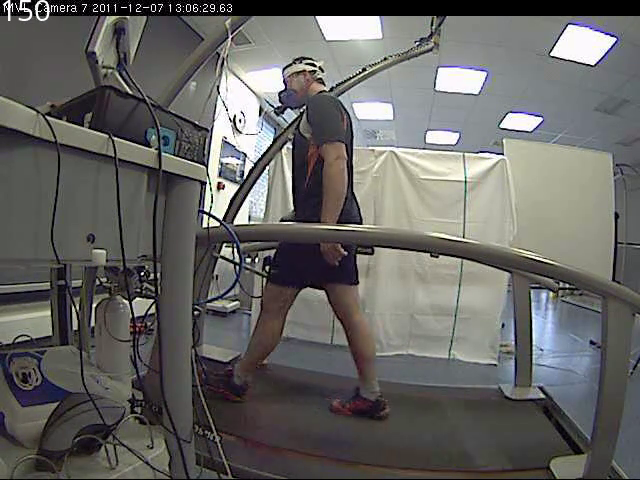
\includegraphics[width=\columnwidth]{./Slike/normal-sv-150.png}
		\caption{Originalna slika}
	\end{subfigure}
	~
	\begin{subfigure}{0.45\columnwidth}
	    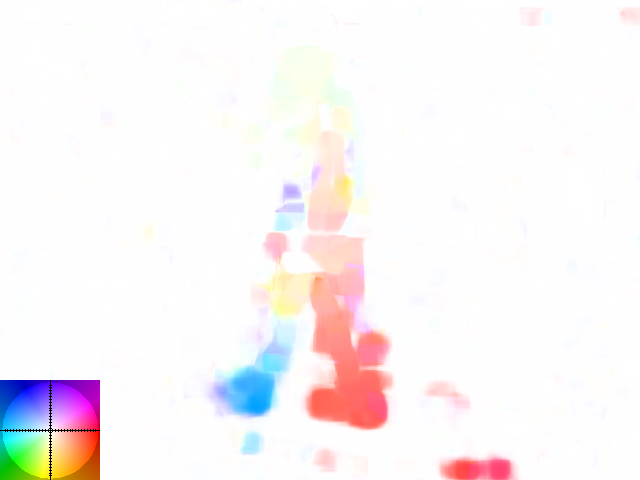
\includegraphics[width=\columnwidth, frame]{./Slike/normal-sv-of-coded-150.png}
		\caption{Slika optičnega toka}
	\end{subfigure}
    \caption[Optični tok za $150$. stransko sliko prve serije testov z legendo barvnega kodiranja]{Optični tok za $150$. stransko sliko prve serije testov z legendo barvnega kodiranja v spodnjem levem kotu. Na sliki uporabljamo standardno barvno kodiranje, povzeto po \cite{baker2011database}. Maksimalna amplituda optičnega toka je na tej sliki znašala \SI{17}{ppf}.}
    \label{fig:opticni-tok-stage1}
\end{figure}

Sledilo je generiranje HOOF deskriptorjev, ki smo jih pred tem optimizirali po postopku, opisanem v poglavju \ref{sec:optimizacija-hoof}. Za parameter smo izbrali $N_{HOOF} = 60 $, ker je dal najbolj optimalne rezultate. Primer HOOF deskriptorjev lahko vidimo na sliki \ref{fig:hoof-znacilke}.

\begin{figure}[!htb]
	\centering
	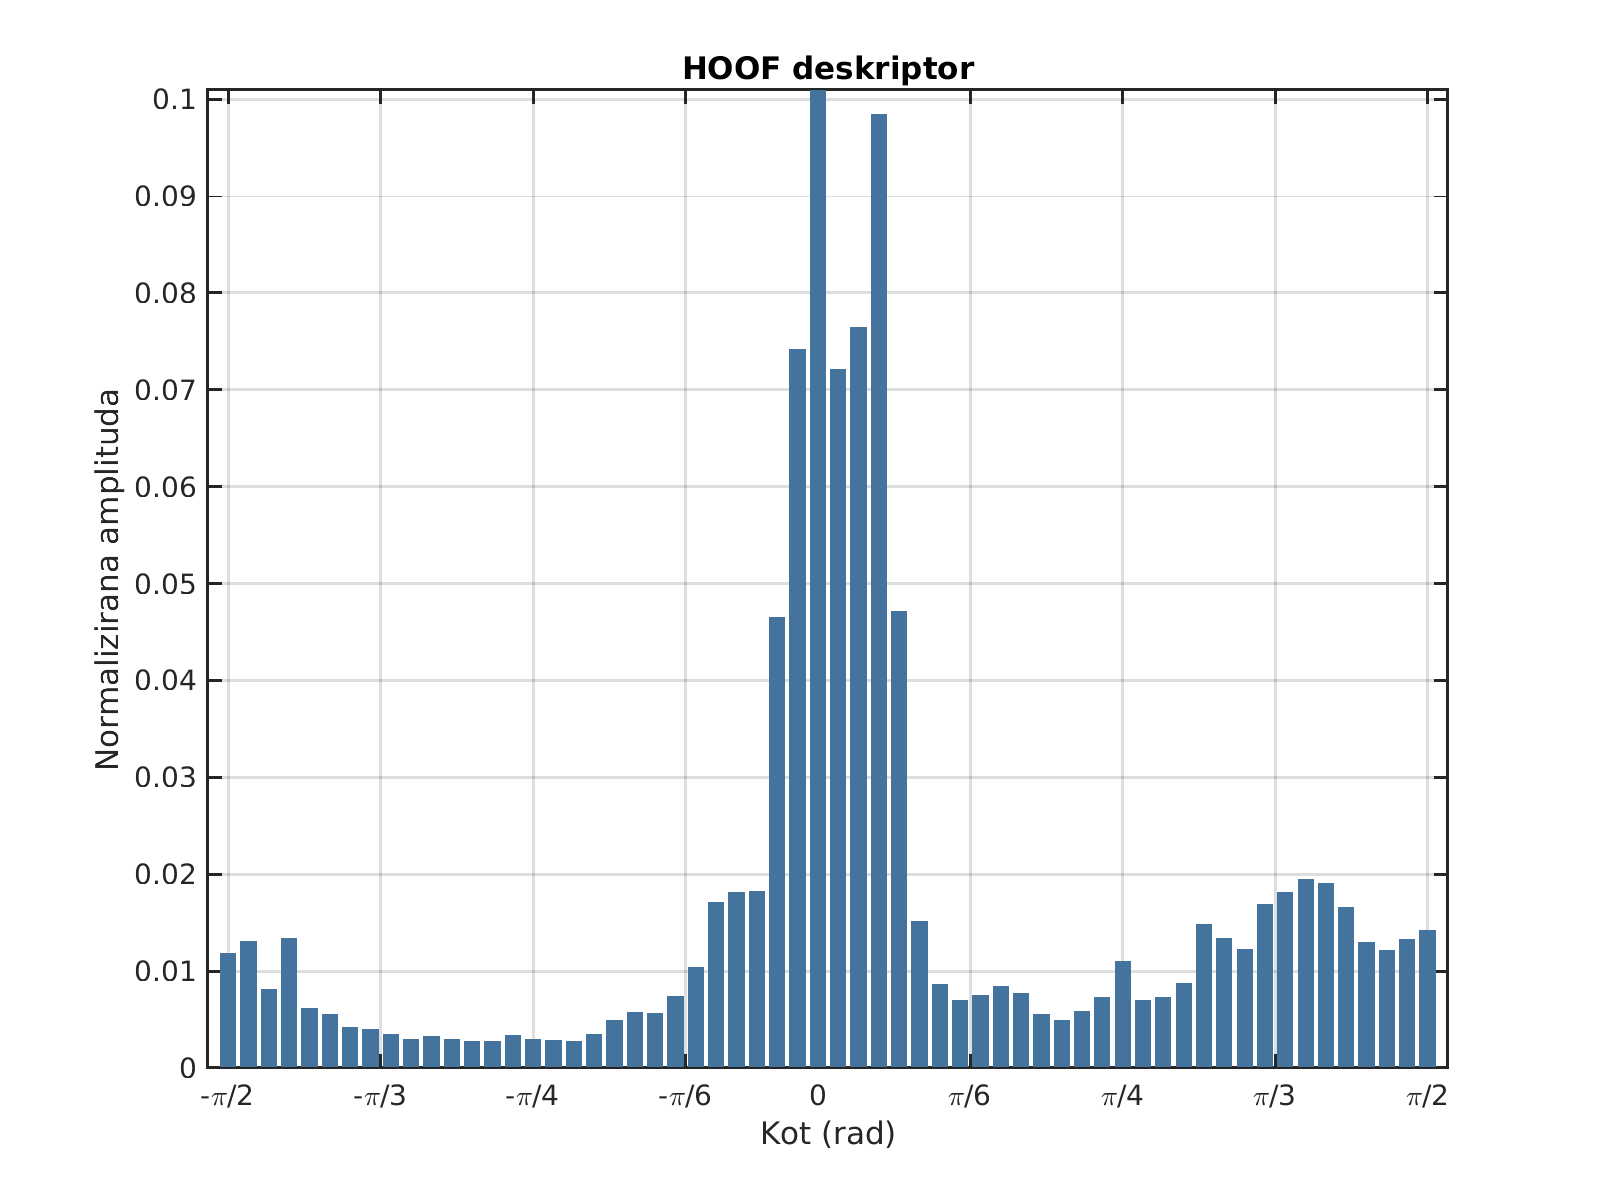
\includegraphics[width=0.75\columnwidth]{./Slike/histogram.png}
	\caption[HOOF deskriptor za 150. RGB sliko prve serije]{HOOF deskriptor za 150. RGB sliko prve serije. Deskriptor smo izračunali iz slike \ref{fig:opticni-tok-stage1}.}
	\label{fig:hoof-znacilke}
\end{figure}

Modele smo učili z metodo podpornih vektorjev $\epsilon$-SVR in jedrom RBF. Regresijske parametre jedra smo optimizirali z metodo mrežnega iskanja. Naučili smo \num{8} elementarnih modelov, ki smo jih razdelili na dve kategoriji: na \textit{hr} modele, ki predvidevajo srčni utrip in modele \textit{eem}, ki predvidevajo porabo energije v \si{\kcal\per\min}. Kategoriji sta nadalje razdeljeni glede na zorni kot kamere: \textit{sv} modeli za stransko kamero in \textit{bv} modeli za hrbtno kamero. Eksperimente smo razširili z vpeljavo zakasnitve med referenčnim fiziološkim parametrom in merjenim parametrom iz slik posnetka. Z eksperimenti, ki so označeni z \textit{lag} kratico, smo preverili predlagano časovno zakasnitev med vzbujanjem in fiziološkim odzivom. 

Generirali smo tudi dodatne modele, in sicer: \textit{crop} modele, \textit{mixed} modele, \textit{track} modele, kjer smo uporabili sledilnik in obremenitvene modele. Ti so deljeni na \textit{scale} modele in \textit{proj} modele.

Vse tipe eksperimentov smo križno testirali glede na enak tip eksperimenta, le z drugim zornim kotom kamere. Uporabljen zorni kot kamere za križno testiranje je v imenih modelov zapisan v oklepajih. Rezultate smo pred testiranjem filtrirali s Kalmanovim filtrom. Uporabljeni parametri so opisani v poglavju \ref{sec:implementacija-kalman}.


\begin{figure}[!htb]
	\centering
	\begin{tikzpicture}
% LAYERS
\pgfdeclarelayer{bg}
\pgfsetlayers{bg,main}
\tikzset{
    between/.style args={#1 and #2}{
         at = ($(#1)!0.5!(#2)$)
    }
}

% NODES
\node (slika) [input] at (0,0) {Področje\\slike $I(x,y)$};

\node (of) [block, right= of slika] {Optični\\ tok $\vec{w}$};
\node (hoof) [block, right= of of] {HOOF\\deskriptor $\vec{x}(t)$};


\node (ucenje) [block, right=of hoof] {$\epsilon$-SVR\\RBF jedro};
\node (kalman) [block, right= of ucenje] {Kalmanov\\filter};


\node (rezultat) [output, right= of kalman] {Rezultat};

% arrows
\draw [arrow] (slika) -- (of);
\draw [arrow] (of) -- (hoof);
\draw [arrow] (hoof) -- (ucenje);
\draw [arrow] (ucenje) -- (kalman);
\draw [arrow] (kalman) -- (rezultat);
\end{tikzpicture}
	\caption[Diagram elemntarnega postopka procesiranja za eksperimente 1. faze]{Diagram elemntarnega postopka procesiranja za eksperimente 1. faze. Izbranemu področju na sliki določimo optični tok }
	\label{fig:diagram-procesiranja-stage1}
\end{figure}

\subsubsection{Določitev zakasnitve fiziološkega odziva}
Na podlagi slike \ref{fig:lag-estimation-stage1} smo ugotovili, da obstaja zakasnitev med spremembo hitrosti tekalne steze in spremembo izbranega fiziološkega parametra. Celoten odziv posameznega fiziološkega parametra je prikazana na sliki \ref{fig:odziv-stage1}.


\begin{figure}[!htb]
	\centering
	\begin{subfigure}[t]{0.45\columnwidth}
		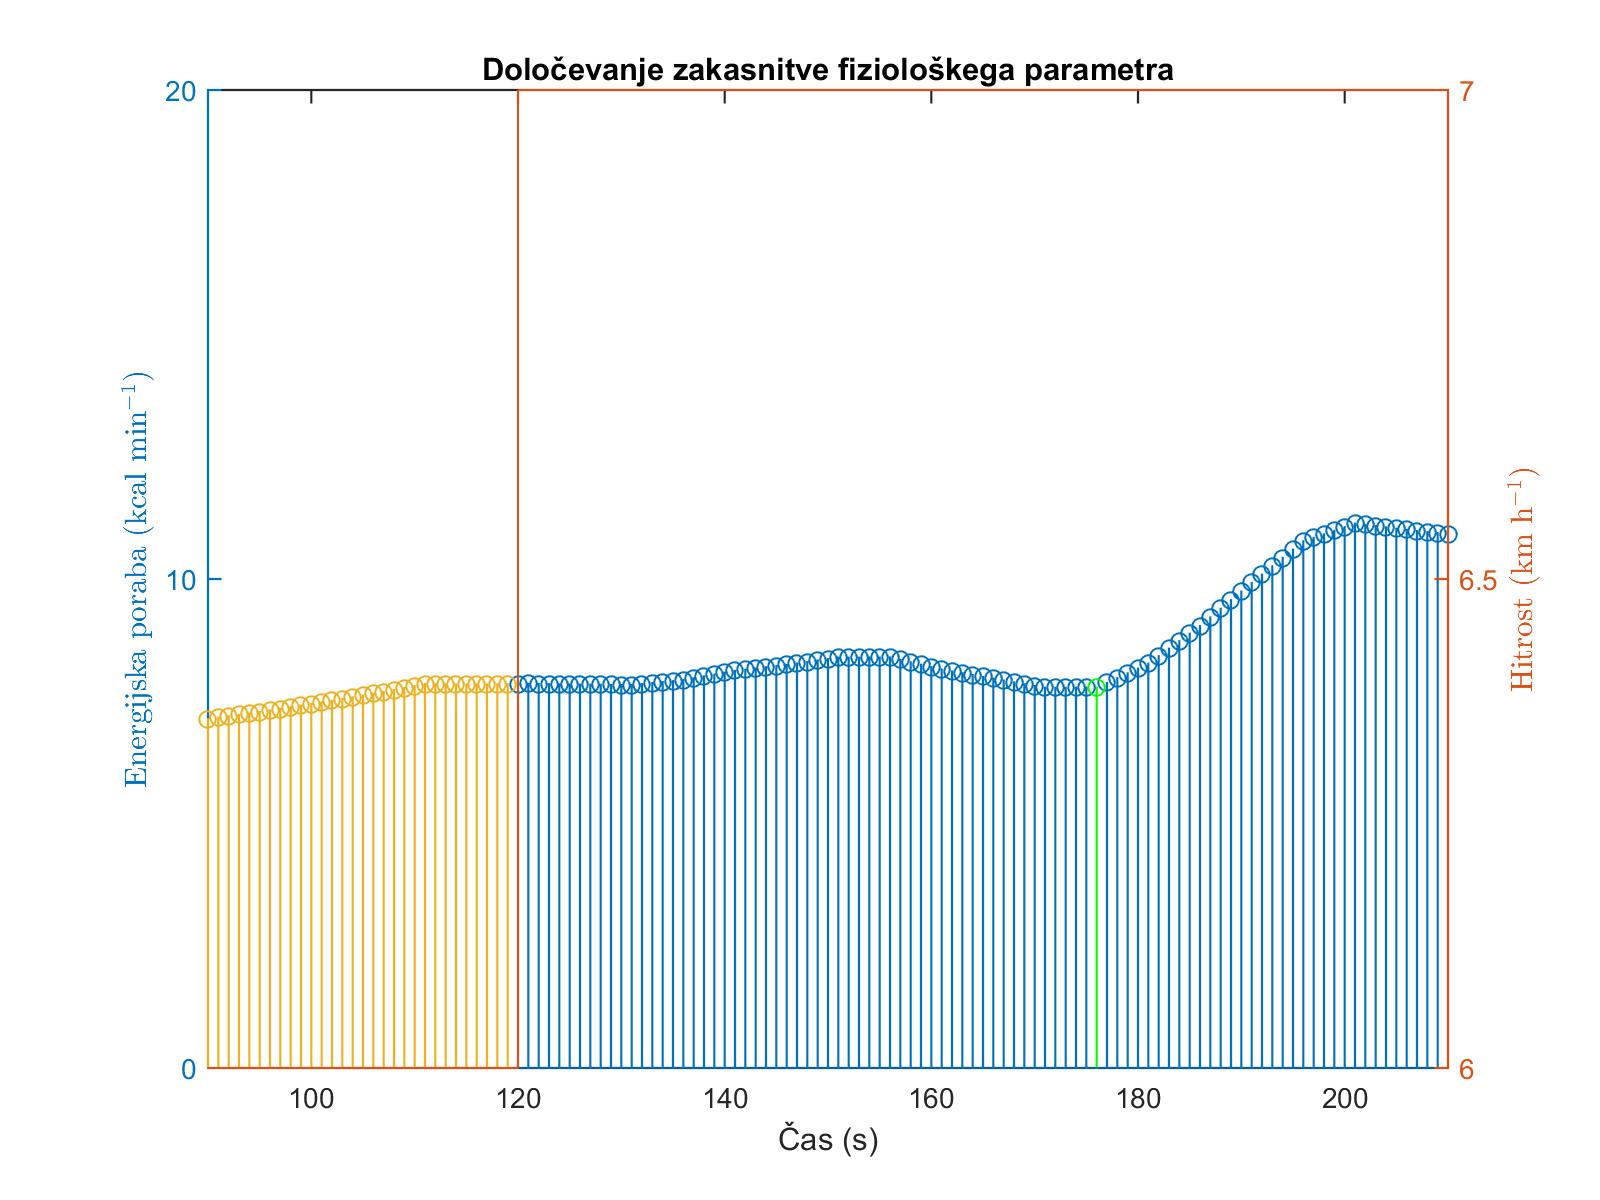
\includegraphics[width=\columnwidth]{./Slike/lag-estimation-train-eem.png}
		\caption{Zakasnitev za energijsko porabo.}
		\label{fig:lag-estimation-train-eem}
	\end{subfigure}
	~
	\begin{subfigure}[t]{0.45\columnwidth}
		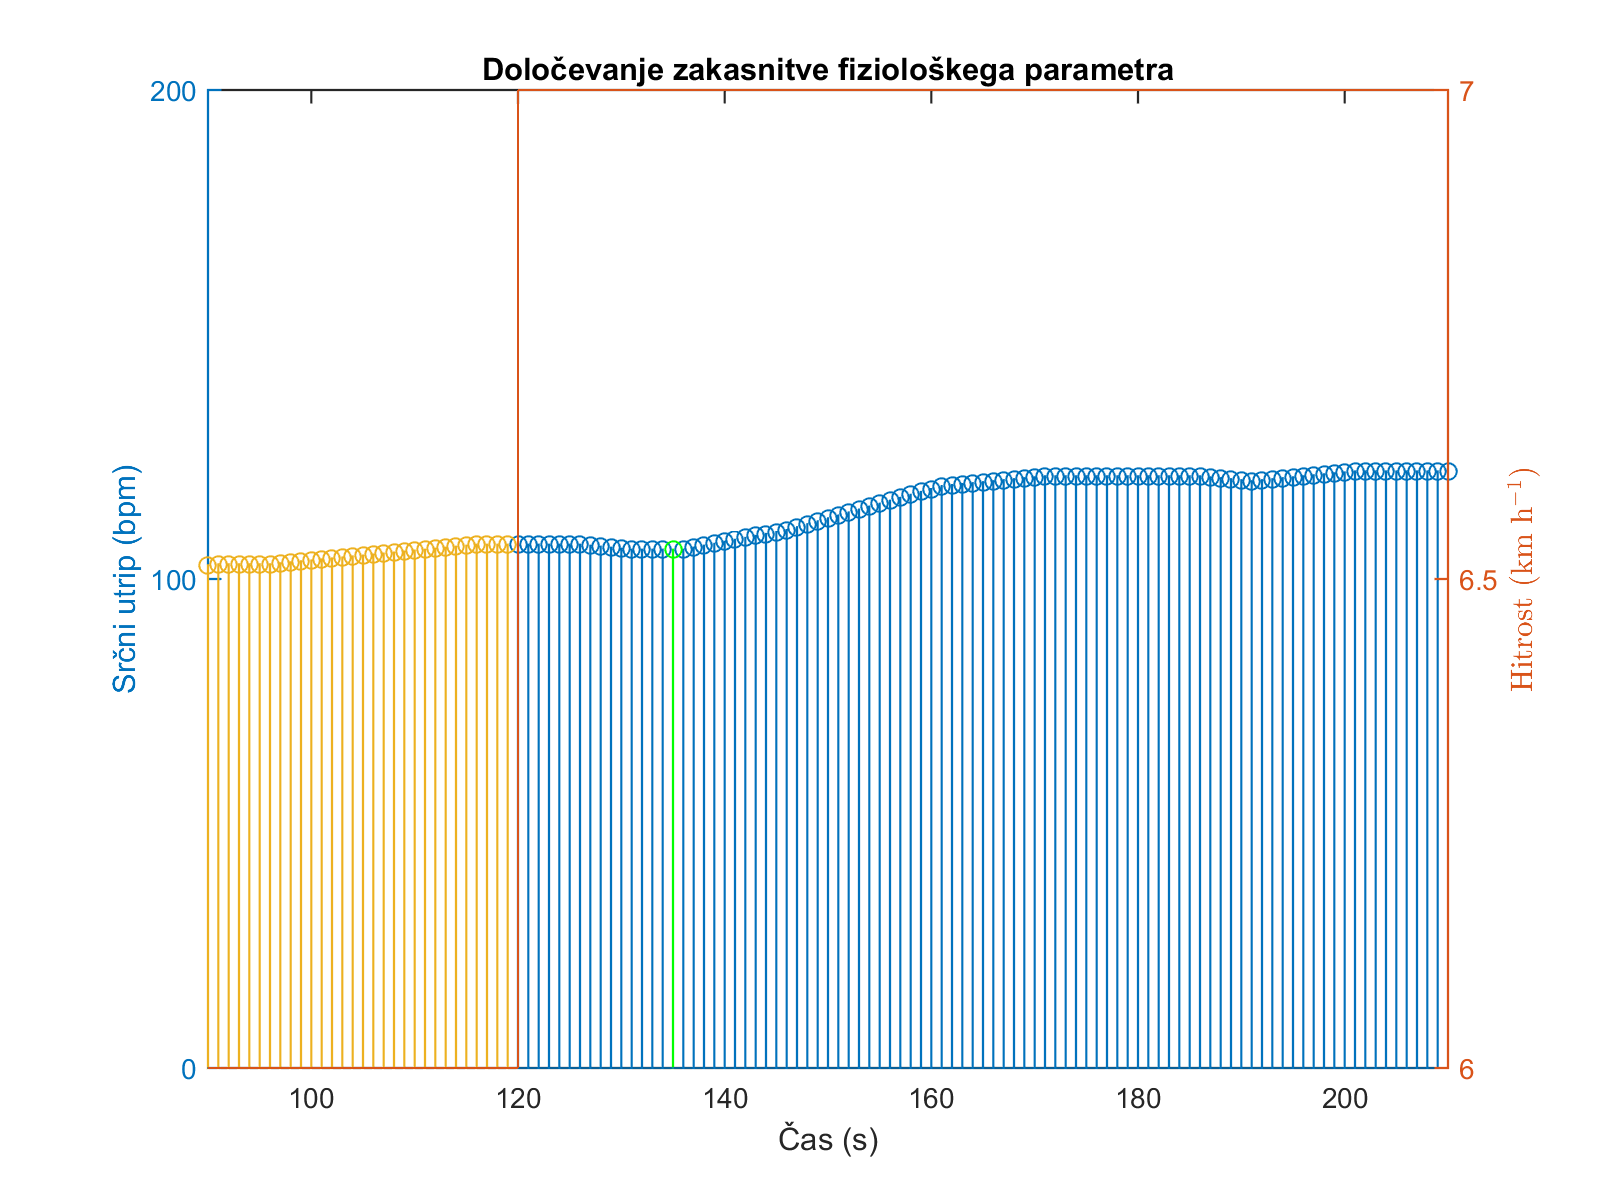
\includegraphics[width=\columnwidth]{./Slike/lag-estimation-train-hr.png}
		\caption{Zakasnitev za srčni utrip.}
		\label{fig:lag-estimation-train-hr}
	\end{subfigure}
	\caption[Prikaz določevanja zakasnitve fiziološkega odziva]{Prikaz določevanja zakasnitve fiziološkega odziva. Na posameznem grafu so prikazani vzorci fiziološkega parametra. Rumena barva označuje vzorce pred spremembo hitrosti tekalne steze, modra pa vzorce po spremembi. Sprememba hitrosti tekalne steze je prikazana z rdečo stopnico. Zeleno obarvani vzorec se nahaja ob trenutku, ko nastane fiziološki odziv.}
	\label{fig:lag-estimation-stage1}
\end{figure}

Zamik za srčni utrip je znašal \SI{15}{\s}. Za energijsko porabo smo izmerili \SI{55}{\s} zamika. Izbrane parametre smo testirali s zakasnitvenimi modeli s kratico \textit{lag}.

Zakasnitev smo določili, kot časovni interval od trenutka spremembe hitrosti tekalne steze do trenutka, ko se je vrednost fiziološkega parametra začela močneje povečevati. Pri tem smo izbrali spremembo hitrosti med prvim in drugim testom, saj je bil signal fiziološkega parametra na tem območju najbolj ustaljen. Kadar je povečevanju dokaj hitro sledil upad, smo smatrali, da do odziva še ni prišlo. Tak primer je prikazan na sliki \ref{fig:lag-estimation-stage1}\subref{fig:lag-estimation-train-eem}), kjer prvemu povečevanju za spremembo hitrosti tekalne steze sledi upad. 


\begin{figure}[!htb]
	\centering
	\begin{subfigure}[t]{0.45\columnwidth}
		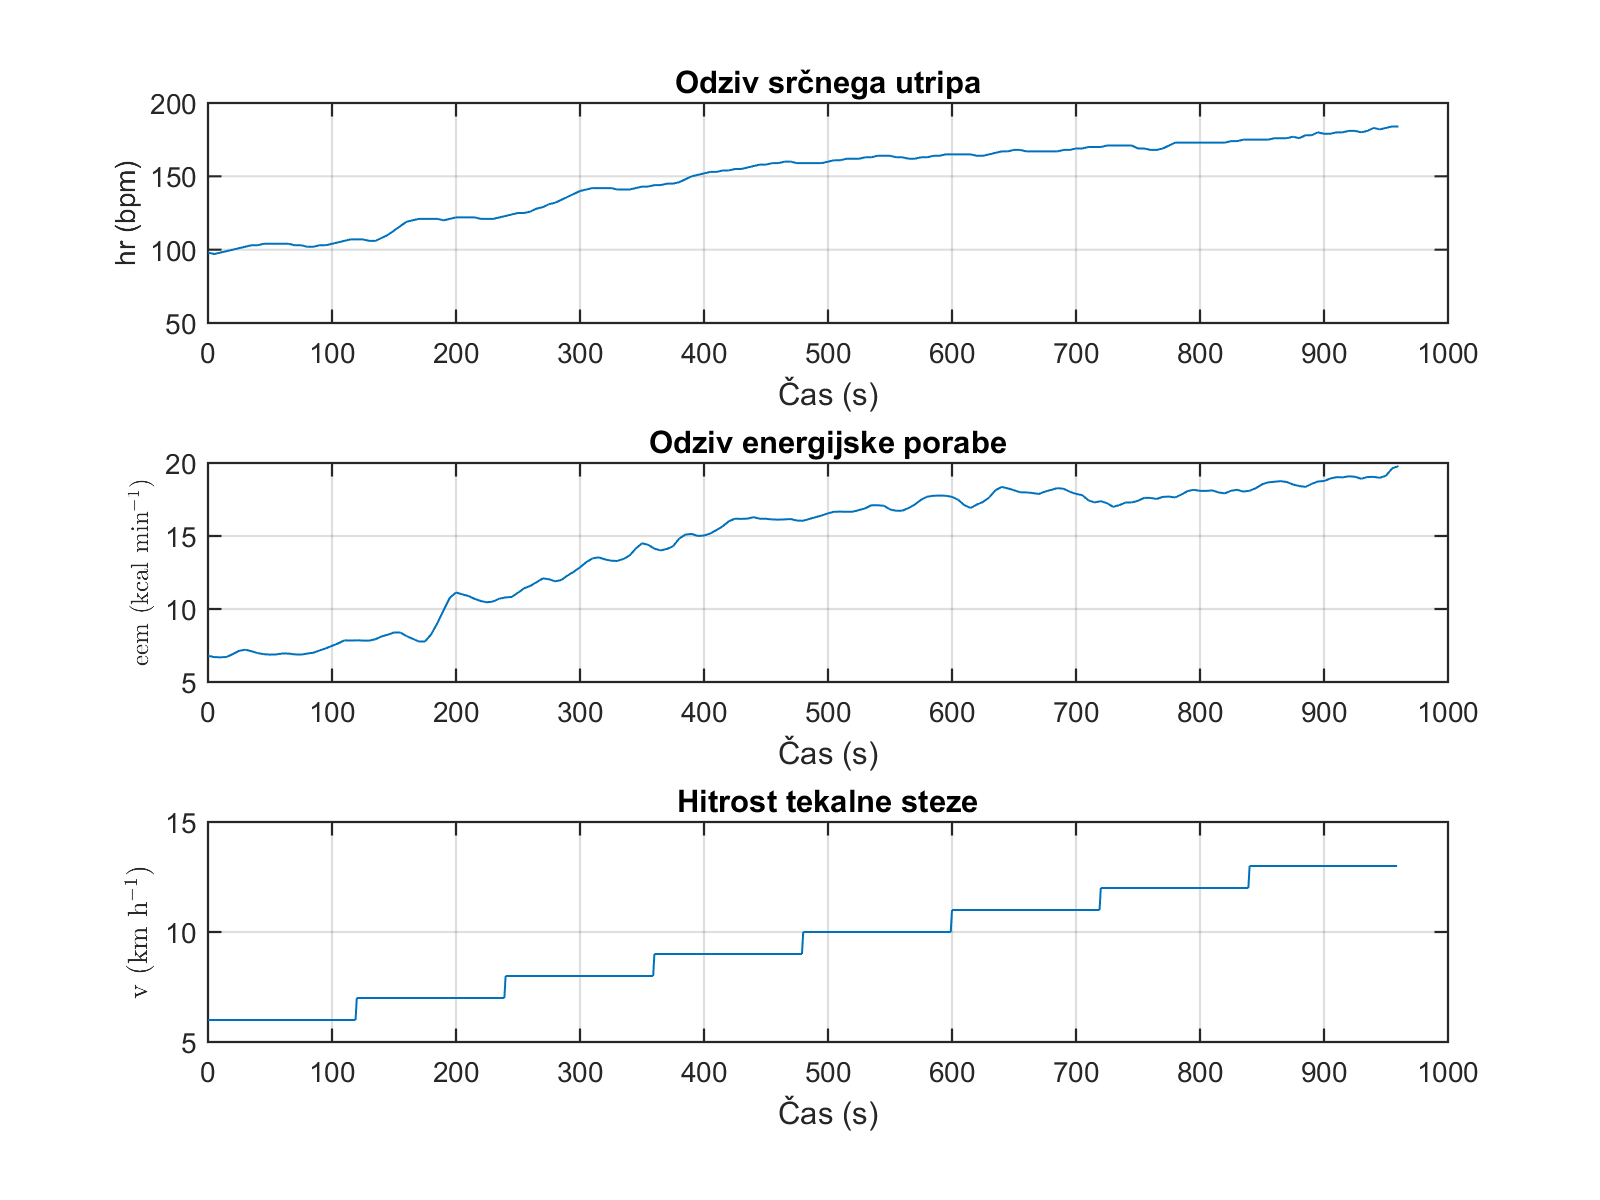
\includegraphics[width=\columnwidth]{./Slike/odziv-train.png}
		\caption{Odziv učnih vzorcev.}
		\label{fig:odziv-ucnih-stage1}
	\end{subfigure}
	~
	\begin{subfigure}[t]{0.45\columnwidth}
		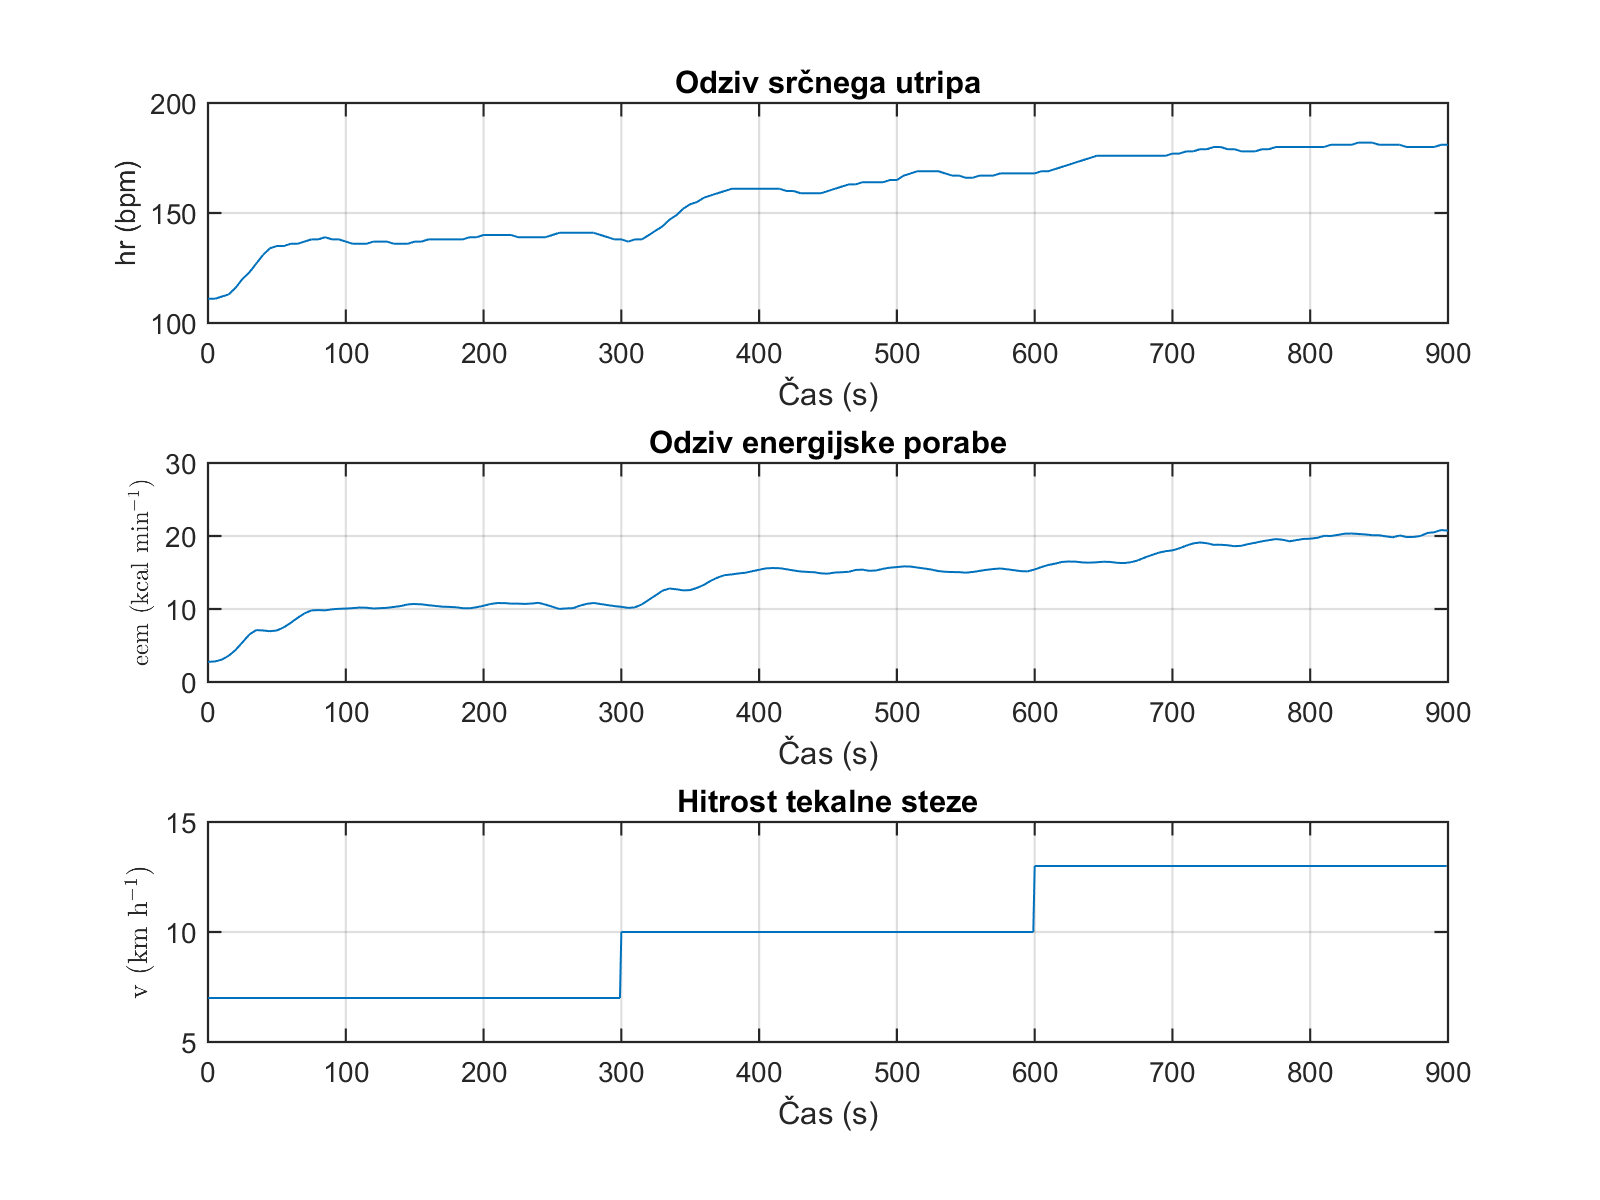
\includegraphics[width=\columnwidth]{./Slike/odziv-test.png}
		\caption{Odziv testnih vzorcev.}
		\label{fig:odziv-testnih-stage1}
	\end{subfigure}
	\caption[Odziv posameznih fizioloških parametrov za obe seriji testov]{Odziv posameznih fizioloških parametrov za obe seriji testov.}
	\label{fig:odziv-stage1}
\end{figure} 


\subsubsection{Ročna določitev področja tarče}
HOOF deskriptorji so v teoriji robustni na šum, saj ta zaradi majhnih amplitud nima vpliva na obliko histograma. Vseeno pa se lahko pojavijo anomalije, ki povečajo amplitudo šuma na raven vrednosti merjenca. Pri tem mislimo predvsem na objekte in osebe v ozadju, ki se premikajo. Temu se lahko preprosto izognemo z določevanjem področja tarče. Ker je bil prizor na posnetkih razmeroma enostaven in ciklično monoton, smo se za preizkus naše hipoteze odločili, da bomo področja najprej določili ročno. Področja smo izbrali tako, da je bil merjenec ves čas skozi posnetek v izbranem področju. Izbrana področja za posamezne posnetke so predstavljena v tabeli \ref{tab:rocna-podrocja}, pri čemer so $h$ dolžina slike $w$ širina slike ter $x$ in $y$ slikovni koordinati.. Vsi nadaljni testi razen, kjer se uporablja sledilnik, temeljijo na izrezanih posnetkih, glede na ta področja.

\begin{table}[!htb]
	\centering
	\begin{tabular}{l l l S[table-format=3] S[table-format=2] S[table-format=3] S[table-format=3]}
		\toprule
		\multicolumn{3}{c}{}& \multicolumn{4}{c}{\textbf{Področje}} \\
		\cmidrule{4-7}
		\textbf{Serija} & \textbf{Pogled} & \textbf{Vrsta} & \thead{$\mathbf{x}$} & \thead{$\mathbf{y}$} & \thead{$\mathbf{w}$} & \thead{$\mathbf{h}$}  \\
		\midrule
		\multirow{3}{*}{1} & \multirow{2}{*}{hrbtni} & RGB & 228 & 43 & 207 & 437 \\
		&& IR & 32 & 10 & 167 & 329 \\
		& stranski & RGB & 179 & 31 & 346 & 420 \\
		\midrule
		\multirow{3}{*}{2} & \multirow{2}{*}{hrbtni} & RGB & 230 & 51 & 228 & 429 \\
		&& IR & 29 & 11 & 181 & 338 \\
		& stranski & RGB & 182 & 33 & 351 & 423 \\
		\bottomrule
	\end{tabular}
	\caption[Ročno izbrana področja tarče za posamezne posnetke]{Ročno izbrana področja tarče za posamezne posnetke. $x$ in $y$ sta koordinati zgornjega levega kota področja. $w$ in $h$ sta širina in dolžina področja.}
	\label{tab:rocna-podrocja}
\end{table}

\subsubsection{Združevanje posnetkov}
V dodatnih \textit{mixed} modelih, smo združili posnetke kamer z različnim zornim kotom. Združeni posnetek je bil po vrstnem redu sestavljen in posnetka stranske kamere in posnetka hrbtne kamere. Pri tem smo uporabili izrezane posnetke glede na ročno določena področja. Z združenim posnetkom smo želeli preveriti vpliv povečevanja informacije o gibanju merjenca zaradi uporabe različnih zornih kotov. 

\subsubsection{Obremenitveni testi}
Z obremenitvenimi testi smo želeli preizkusiti robustnost našega postopka. Opravili smo dve vrsti testov, in sicer: \textit{scale} teste in \textit{proj} teste. Pri \textit{scale} testih smo posnetke zmanjšali za \SI{50}{\%}. S tem smo simulirali večjo oddaljenost merjenca od kamere in tako preverili teoretično invariantnost HOOF deskriptorjev glede na skalo.

Z vnašanjem projektivne transformacije v posnetke smo s \textit{proj} testi preizkušali robustnost celotnega postopka na deformacije slike, ki jo lahko vnašajo leče kamere. Projektivno transformacijo smo izvedli s pomočjo matlabovih funkcij \texttt{fitgeotrans} in \texttt{imwarp}. Za vhodne točke smo izbrali robove posamezne slike zaporedja. Za izhodne točke smo izbrali vrednosti v tabeli \ref{tab:projective}, pri čemer so $h$ dolžina slike, $w$ širina slike ter $x$ in $y$ slikovni koordinati.

\begin{table}[!htb]
	\centering
	\begin{tabular}{l S[table-format=1.3] S[table-format=1.3] }
		\toprule
		\thead{Točka} & \thead{$\mathbf{x~[\times w]}$} & \thead{$\mathbf{y~[\times h]}$} \\
		\midrule
		$P_0$ & 0 & 0.25 \\
		$P_1$ & 1 & 0 \\
		$P_2$ & 0.125 & 0.75 \\
		$P_3$ & 0.875 & 0.875 \\
		\bottomrule
	\end{tabular}
	\caption[Tabela pozicij robov transformirane slike]{Tabela pozicij robov transformirane slike. $h$ je dolžina slike, $w$ širina slike ter $x$ in $y$ slikovni koordinati.}
	\label{tab:projective}
\end{table}


\begin{figure}[!htb]
	\centering
	\begin{subfigure}[t]{0.45\columnwidth}
		\centering
		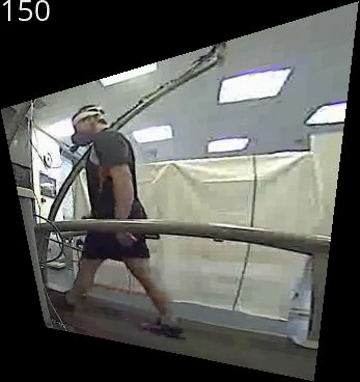
\includegraphics[width=0.6\columnwidth]{./Slike/projective-sv-150.png}
		\caption{Stranska slika}
	\end{subfigure}
	~
	\begin{subfigure}[t]{0.45\columnwidth}
		\centering
		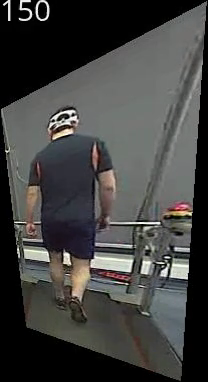
\includegraphics[width=0.6\columnwidth]{./Slike/projective-bv-150.png}
		\caption{Hrbtna slika}
	\end{subfigure}
	\caption[Primer projektivne transformacije 150. slike posnetka iz prve serije]{Primer projektivne transformacije 150. slike posnetka iz prve serije. Prikazani sta stranska in hrbtna transformirana slika. Transformirali smo slike \ref{fig:primer-posnetka-rgb}.}
	\label{fig:projective}
\end{figure}


\subsubsection{Sledenje merjencem}\label{sec:tracking}
Obstaja veliko ekipnih športov, kjer sodeluje več igralcev. Ker so vsi vidni na vsaki sliki zaporedja posnetka, je nujno, da v naš sistem uvedemo funkcionalnost sledenja. S sledenjem na tekalni stezi smo preverili delovanje te funkcionalnosti. Rezultati, ki vsebujejo korak sledenja imajo kratico \textit{tr}. Primer sledenja je prikazan na sliki \ref{fig:sledenje}.

\begin{figure}[!htb]
	\centering
	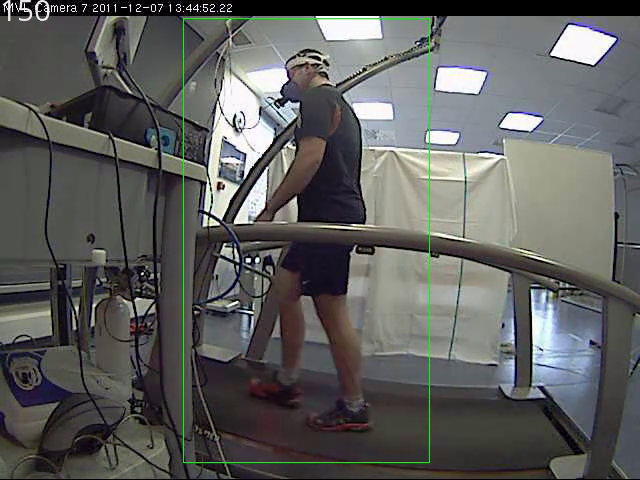
\includegraphics[width=0.6\columnwidth]{./Slike/normal-sv-test-kcf2.png}
	\caption[Sledenje merjencu s KCF na stranski sliki.]{Sledenje merjencu s KCF na stranski sliki. Prikazana je 150. slika RGB posnetka druge serije. Zeleni okvir prikazuje področje, ki ga je detektiral sledilnik.}
	\label{fig:sledenje}
\end{figure} 

Za sledenje smo uporabili KCF sledilnik, ki je implementiran v OpenCV knjižnici. Izbiro sledilnika smo opredelili že v poglavju \ref{sec:testiranje-sledilnikov-za-opticni-tok}. Pri sledenju smo uporabili sledeče parametre: pasovna širina gaussovega jedra $0.2$, linearni interpolacijski faktor za adaptacijo $0.075$, regularizacijski faktor $0.01$, največja velikost obliža (ang. Patch) $6400$, prostorska pasovna širina $0.0625$, aktivirano skaliranje značilk za izboljšanje hitrosti procesiranja, razcepljeni učni koeficienti na dve matrike, dekativirano zavijanje (ang. wrapping) okoli vrednosti jedra, nekompresirani deskriptorji za sivinske slike in kompresirani za barvne slike, aktivirana PCA metoda za kompresijo značilk, velikost kompresije $2$ in  stopnja učenja kompresije $0.15$.

KCF sledilnik smo inicializirali z ročnim obkroževanjem področja tarče na prvi sliki vsakega posnetka. Področja tarče, ki jih je izbral sledilnik, smo uporabili za izrezovanje področij merjenca iz slik optičnega toka. HOOF deskriptorje smo izračunali le na izbranem področju. 



\subsubsection{Simulacija vibracij kamere}
Kadar uporabljamo ročne kamere, pogosto pride do tresenja. Vibracije smo simulirali z majhnimi naključnimi premiki in rotacijo posameznih slik iz video zaporedja. Vsako sliko smo transformirali z Evklidsko transformacijo. Pri tem smo translacijo omejili na \SI{4}{\%} velikosti slike. Rotacija je bila omejena na \SI{0.13}{rad}. 

Translacijo in rotacijo smo filtrirali še s Kalmanovim filtrom, tako da smo dobili bolj realistično simulacijo. Za Kalmanov filter smo uporabili enak model, kot je predstavljen v poglavju \ref{sec:kalmanov-filter}. Začetne variance filtra smo določili empirično tako, da smo dobili čimbolj realistične rezultate. Varianca šuma merilnega modela je znašala $\sigma_\vec{z}^2=1024$, variancal šuma modela gibanja pa $\sigma_\vec{x}^2=2$. Za kovariančno matriko predikcije smo uporabili varianco $\sigma_\vec{P}^2=2$.

S simulacijo vibracij smo naredili obremenitveni test za modele z vključenim sledilnikom. Rezultati so anotirani s \textit{sh} kratico. Primer delovanja sledilnika je prikazan na sliki \ref{fig:vibracije}.

\begin{figure}[!htb]
	\centering
	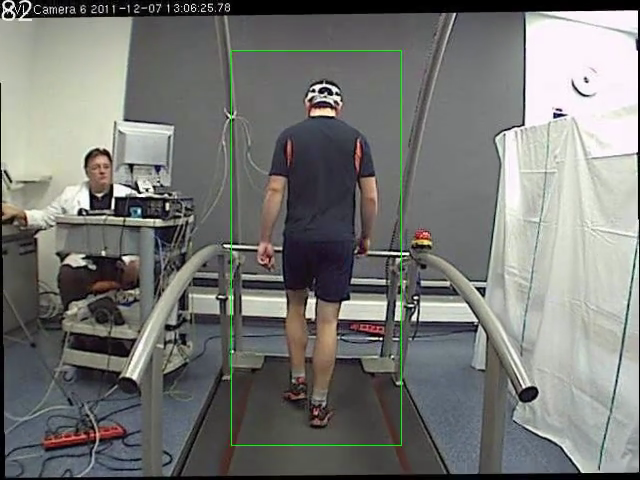
\includegraphics[width=0.6\columnwidth]{./Slike/shake-bv-train-kcf2.png}
	\caption[Sledenje merjencu na tresočem posnetku]{Sledenje merjencu na tresočem posnetku. Prikazana je 82. slika hrbtnega RGB posnetka prve serije. Zeleni okvir prikazuje področje, ki ga je detektiral KCF sledilnik.}
	\label{fig:vibracije}
\end{figure} 








\subsection{Terenski eksperimenti squash igre}
Pri terenskih eksperimentih smo snemali dve squash igri z enim setom z RaspberryPi in RaspiCam napravo v resoluciji  $1920 \times 1080$. Zaradi nezadovoljivih podatkov druge igre, smo za učenje in testiranje modelov uporabili le prvo igro. Igralcem smo merili srčni utrip s kontaktnimi senzorji. 

Prvega igralca prve igre  (starost: 45 let, velikost: \SI{176}{\cm}, teža: \SI{68}{\kg}, spol: male, $hr_{tmax}$: \SI{179}{bpm}, $hr_{r}$: \SI{45}{bpm}) smo uporabili za učne vzorce. Drugega igralca (starost: 17 let, višina: \SI{178}{\cm}, teža: \SI{66}{\kg}, spol: male, $hr_{tmax}$: \SI{203}{bpm}, $hr_{r}$: \SI{50}{bpm}) smo uporabili za testne vzorce. 

\subsubsection{Razširitev HOOF deskriptorja}
Chaudhry et al. \cite{chaudhry2009histograms} predlaga uporabo histogramov orientiranega optičnega toka (HOOF) za estimacijo gibanja. Vendar pa smo v terenskih testiranjih ugotovili, da njihova uporaba v realnih okoliščinah ni zadovoljiva. HOOF deskriptorju smo pripeli HAFA deskriptor in tako dobili razširjeni deskriptor HOOF-HAFA, ki v splošnem daje boljše rezultate, kot je bilo prikazano v poglavju \ref{sec:razsiritev-hoof-rezultati}. Primer deskriptorja je viden na sliki \ref{fig:hoof-hafa}.

\begin{figure}[!htb]
	\centering
	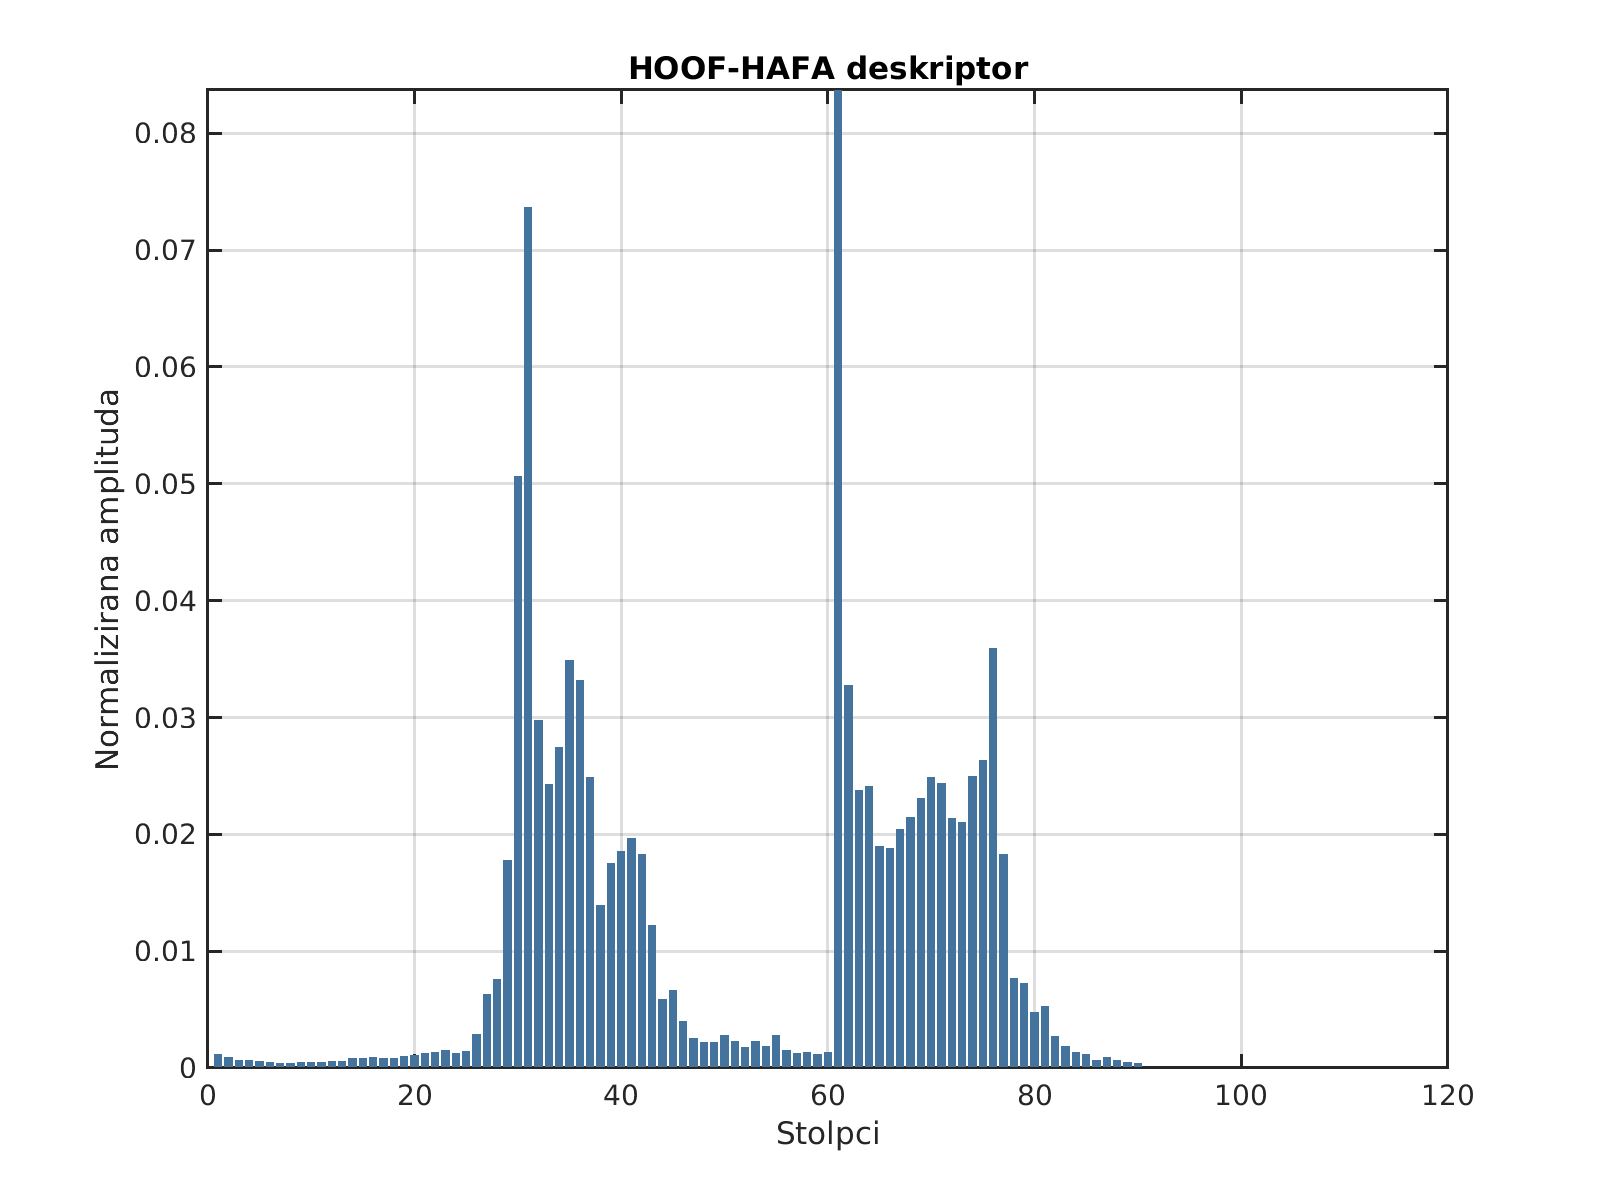
\includegraphics[width=0.6\columnwidth]{./Slike/hoof-hafa-squash-276.png}
	\caption[HOOF-HAFA deskriptor za 276. sliko učnih vzorcev]{HOOF-HAFA deskriptor za 276. sliko učnih vzorcev. Deskriptor se ujema s sliko \ref{fig:sledenje-squash}.}
	\label{fig:hoof-hafa}
\end{figure}

\subsubsection{Postopek procesiranja}
Za določitev področja posameznega igralca smo uporabili KCF sledilnik. Kadar sledilnik ni uspel najti objekta zanimanja, je bilo področje prazno, zato so bile vse vrednosti HOOF-HAFA deskriptorjev $0$. To se je zgodilo v primerih, ko je tarča izginila iz vidnega polja kamere ali pa ko sledilnik ni več deloval. Zaradi teh težav smo sledenje nadzorovano reinicializirali vsake \SI{3}{\s}. S tem smo zagotovili razumne sledilne rezultate. Zaradi prevelike resolucije posnetkov, smo morali za pravilno delovanje sledilnika posnetke skalirati na \SI{25}{\%} prvotne velikosti. Rezultate sledenja smo nato morali transformirati nazaj na originalno resolucijo. Primer sledenja je prikazan na sliki \ref{fig:squash}\subref{fig:sledenje-squash})

\begin{figure}[!htb]
	\centering
	\begin{subfigure}[t]{0.45\columnwidth}
		\centering
		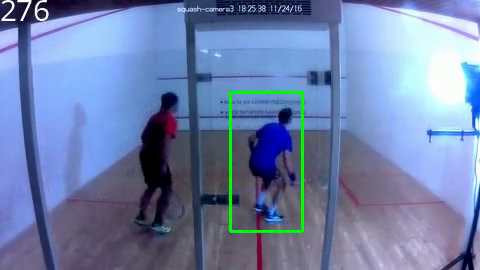
\includegraphics[width=\columnwidth]{./Slike/squash-tracked.png}
		\caption{Slika sledenja.}
	    \label{fig:sledenje-squash}
	\end{subfigure}
	~
	\begin{subfigure}[t]{0.45\columnwidth}
		\centering
		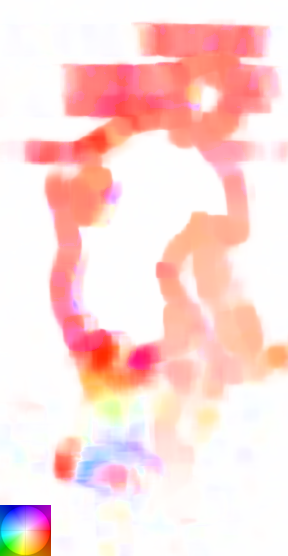
\includegraphics[width=0.6\columnwidth, frame]{./Slike/stage1-squash-flo-corrected.png}
		\caption{Slika optičnega toka.}
		\label{fig:of-squash}
	\end{subfigure}
	\caption[Slika sledenja in optičnega toka za igralca prve igre terenskih squash eksperimentov]{Slika sledenja in optičnega toka za igralca prve igre terenskih squash eksperimentov. Sledili smo modremu igralcu, ki smo ga uporabili za učne vzorce. Zeleni okvir na sliki \subref{fig:sledenje-squash}) prikazuje področje detekcije 276. slike posnetka. Korespondečni optični tok področja je prikazan na sliki \subref{fig:of-squash} z legendo barvnega kodiranja v spodnjem levem kotu. Na sliki uporabljamo standardno barvno kodiranje, povzeto po \cite{baker2011database}. Maksimalna amplituda optičnega toka je na tej sliki znašala \SI{31}{ppf}. }
	\label{fig:squash}
\end{figure}

Izmerjeni srčni utrip smo filtrirali z Gaussovim filtrom s standardnim odklonom \num{16}. S tem smo preprečili učenje na šumnih podatkih. Srčni utrip je bil individualiziran na parametre učnega igralca s pretvorbo v energijsko porabo po enačbi \eqref{eq:charlot}. Rezultate smo nato z isto enačbo pretvorili nazaj v srčni utrip s parametri testnega igralca. S tem smo omogočili učenje na enem in testiranje na drugem igralcu. 

Po določevanju optičnega toka (slika \ref{fig:squash}), smo uporabili HOOF-HAFA deskriptorje, katerih značilke smo skalirali na intervalu $[-1,1]$. Učili smo s postopkom \esvr in jedrom RBF. Za terenske eksperimente Kalmanovega filtra nismo uporabili. Ker je bil Gaussov filter uporabljen pri predprocesiranju podatkov, smo enak filter uporabili tudi za filtriranje izhodov modela.

\begin{figure}[!htb]
	\centering
	\begin{tikzpicture}
% LAYERS
\pgfdeclarelayer{bg}
\pgfsetlayers{bg,main}
\tikzset{
    between/.style args={#1 and #2}{
         at = ($(#1)!0.5!(#2)$)
    }
}

% NODES
\node (slika) [input] at (0,0) {Slika\\$I(x,y)$};
\node (tracker) [block, right= of slika] {KCF\\sledilnik};
%\node (tarca) [block, right= of tracker] {Področje\\tarče};

\node (of) [block, right= of tracker] {Optični\\tok $\vec{w}$};
\node (hoof) [block, right= of of] {HOOF-HAFA\\deskriptorji\\$\vec{x}(t)$};


\node (ucenje) [block, right=of hoof] {\esvr\\RBF};
\node (kalman) [block, right= of ucenje] {Gaussov\\filter};


\node (rezultat) [output, right= of kalman] {Rezultat};

% arrows
\draw [arrow] (slika) -- (tracker);
\draw [arrow] (tracker) -- (of);
%\draw [arrow] (tarca) -- (of);
\draw [arrow] (of) -- (hoof);
\draw [arrow] (hoof) -- (ucenje);
\draw [arrow] (ucenje) -- (kalman);
\draw [arrow] (kalman) -- (rezultat);
\end{tikzpicture}
	\caption[Diagram procesiranja terenskih eksperimentov 1. faze]{Diagram procesiranja terenskih eksperimentov 1. faze. Področju, ki smo ga dobili s KCF sledinikom, smo določili optični tok. Sledilo je učenje na HOOF-HAFA deskriptorjih, Rezultate smo filtrirali s Gaussovim filtrom.}
	\label{fig:diagram-procesiranja-field-stag1}
\end{figure}

















\subsection{Detekcija dihanja}
Za prikaz splošne uporabnosti elementarnega postoka iz poglavja \ref{sec:elementarni-postopek}, smo ga uporabili za detekcijo dihanja. Za razliko od uporabe postopka v športu, lahko detekcijo dihanja uporabljamo za medicinske namene, v skrbi za starejše ali pri nadzornih kamerah. Koncept optičnega merjenja nam omogoča, da aplikacijo uporabimo z daljših razdalj, dokler nam optični sistem to omogoča. 

Seveda obstaja že kar nekaj aplikacij monitoringa pacientov s pomočjo računalniškega vida. Naša glavna motivacija je bilo testiranje predlagane metode na drugačnem problemu.

\subsubsection{Pridobivanje podatkov}
Za testiranje detekcije dihanja smo posneli video moškega merjenca, starosti 42 let z diagnozo spalne apneje. Snemanje se je začelo ob 4:45 zjutraj med spanjem merjenca in je trajalo 30 min. Prostor smo osvetlili z \SI{60}{w} bližnje-infrardečim (NIR) osvetljevalnikom. Snemali smo z RaspberryPi RaspiCam  napravo (NIR verzija, brez filtra za blokiranje NIR). Hitrost snemanja je bila \SI{25}{fps}, ki smo jo zmanjšali na \SI{10}{fps} v predprocesiranju videa. Ker je dihanje počasen proces, smo z zmanjševanjem hitrosti izboljšali SNR v pridobljenem optičnem toku. Pri snemanju smo uporabili širokokotno M12 lečo z goriščno razdaljo \SI{1.8}{mm}. Snemalna aparatura je bila oddaljena približno \SI{2}{m} od opazovanega subjekta. Primer slike posnetka je prikazan na sliki \ref{fig:dihanje-orig}.

\begin{figure}[htb]
	\centering
	\begin{subfigure}[t]{0.45\columnwidth}
		\centering
		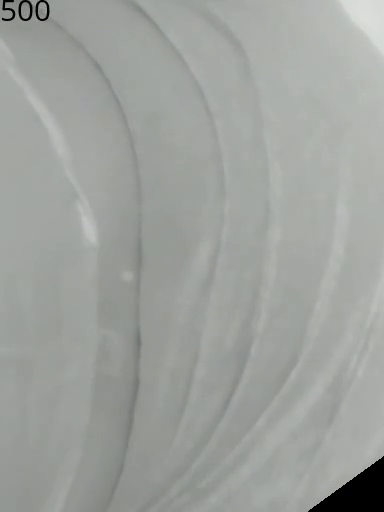
\includegraphics[width=0.75\columnwidth]{./Slike/breathtest-500.png}
		\caption{IR slika dihanja.}
		\label{fig:dihanje-orig}
	\end{subfigure}
	~
	\begin{subfigure}[t]{0.45\columnwidth}
		\centering
		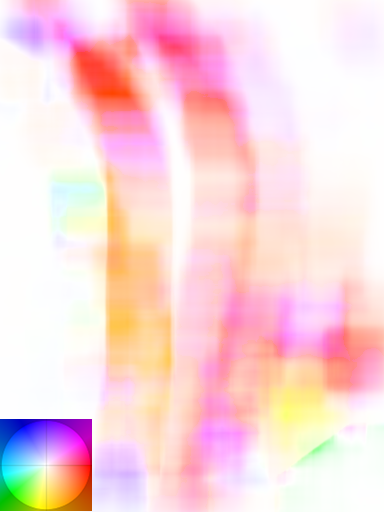
\includegraphics[width=0.75\columnwidth, frame]{./Slike/breathtest-flow-coding.png}
		\caption{Optični tok dihanja.}
		\label{fig:dihanje-of}
	\end{subfigure}
	~
	\begin{subfigure}[t]{0.45\columnwidth}
		\centering
		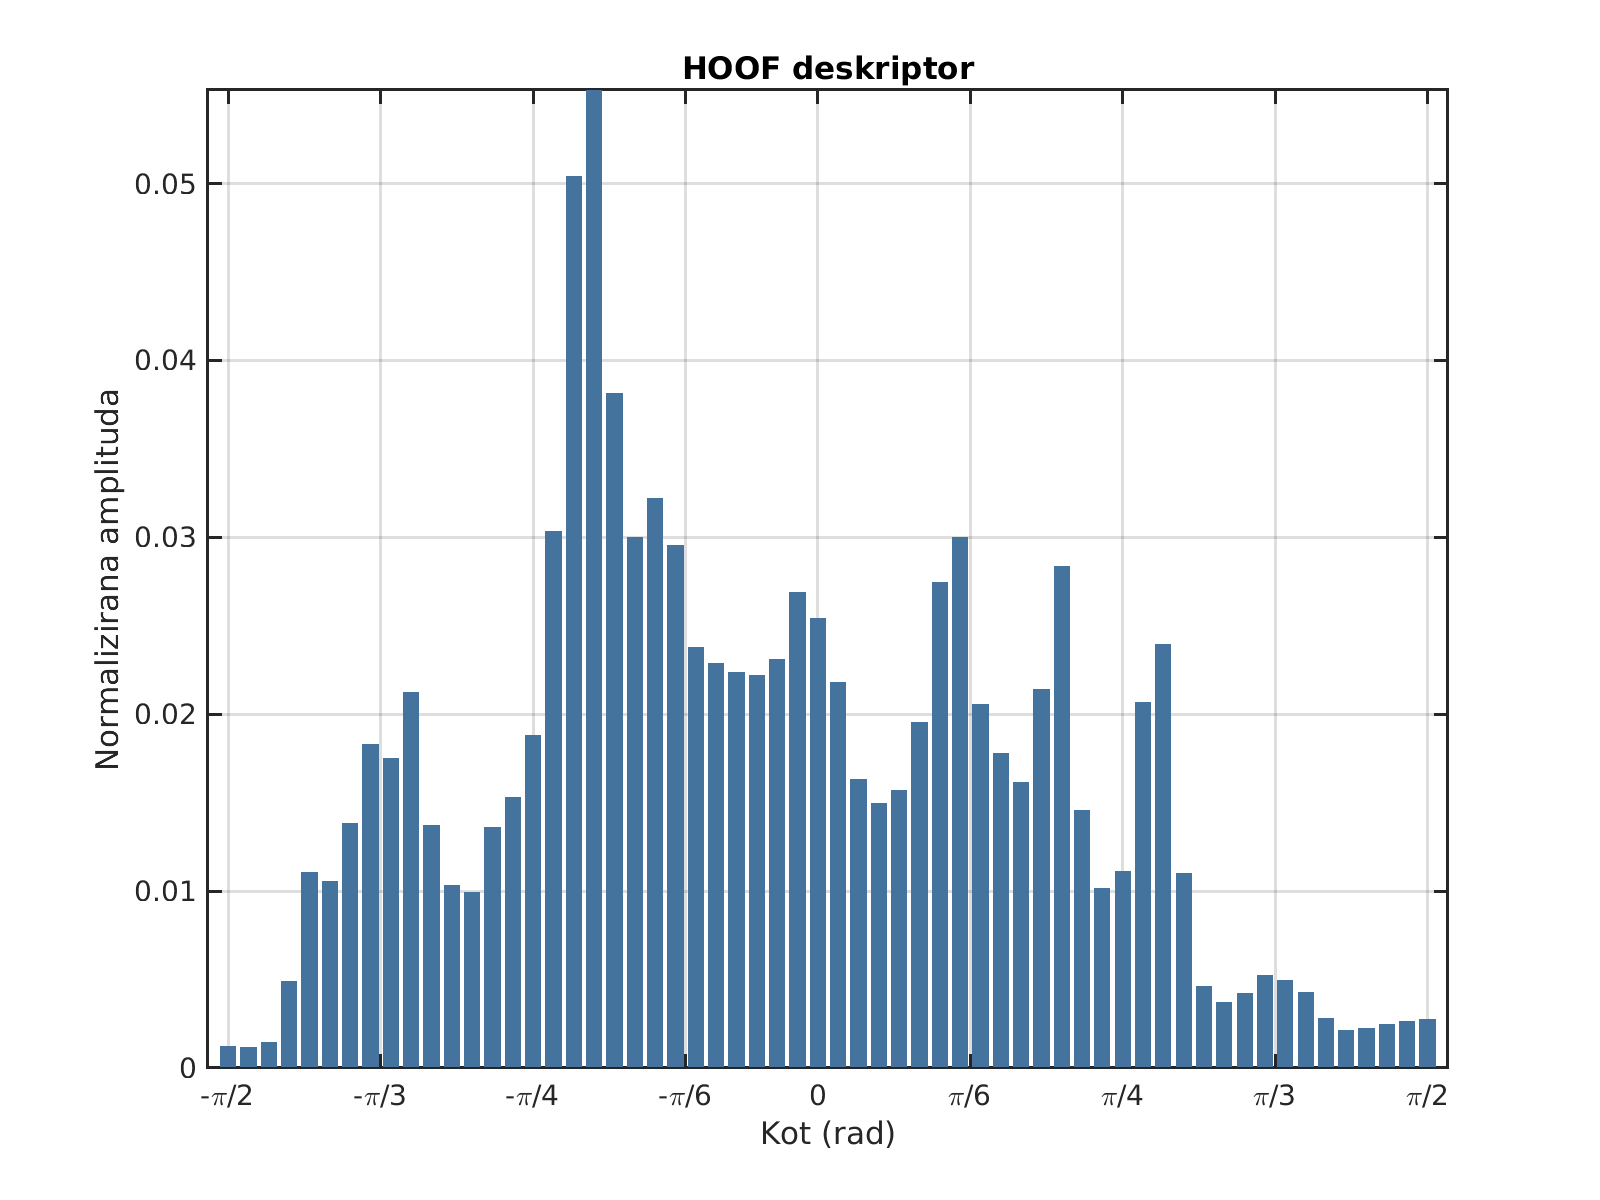
\includegraphics[width=\columnwidth]{./Slike/breathtest-histogram.png}
		\caption{HOOF histogram.}
		\label{fig:dihanje-hist}
	\end{subfigure}
	\caption[Originalna IR slika dihanja, njen optični tok in HOOF histogram]{Originalna IR slika dihanja, njen optični tok in HOOF histogram Prikazana je 500. slika učnih vzorcev. Optični tok ima z legendo barvnega kodiranja v spodnjem levem kotu. Na sliki uporabljamo standardno barvno kodiranje, povzeto po \cite{baker2011database}. Maksimalna amplituda optičnega toka je na tej sliki znašala \SI{1}{ppf}.}
	\label{fig:dihanje}
\end{figure} 

\subsubsection{Referenčni podatki}
Za pridobitev referenčnih podatkov smo snemali tudi zvok z avdio modulom za RaspberryPi. Mikrofon smo postavili v neposredno bližino merjenca. Zvok smo sinhronizirali z video posnetkom. Detekcije dihanja so predstavljale visoko amplitudo zvoka. Dobljene detekcije smo pregledali z operaterjem in potrdili, da korespondirajo z dejanskim dihanjem na avdio posnetku. Detekcije dihanja smo prevzorčili na \SI{10}{Hz}, da so se skladale s frekvenco vzorčenja video posnetka.

\subsubsection{Procesiranje}\label{sec:data-preprocessing}
Opazovali smo področje subjektovega hrbta. Subjekt je ležal obrnjen navzdol. Področje je bilo veliko $384 \times 512$ slikovnih elementov in je pokrivalo približno $2/3$ hrbta. To je bil edini del slike, ki smo ga uporabili.

Iz posnetka smo izbrali dva zaporedja slik s trajanjem \SI{5}{min}. Prvo zaporedje smo uporabili za učenje, drugo pa za testiranje. Pri uporabi optičnega toka smo spremenili parameter velikost okna na $64$. Iz optičnega toka smo izračunali HOOF histograme. Njihove značilke smo normirali na intervalu $[-1,1]$. Učili smo z C-SVC razvrščevalnikom in RBF jedrom, pri tem pa uporabili optimizacijo parametrov. Za določitev uspešnosti delovanja smo problem formulirali kot problem binarnega razvrščanja z razredoma ``diha'' in ``ne diha''. Rezultatov nismo filtrirali.

\begin{figure}[htb]
	\centering
	\begin{tikzpicture}
% LAYERS
\pgfdeclarelayer{bg}
\pgfsetlayers{bg,main}
\tikzset{
	between/.style args={#1 and #2}{
		at = ($(#1)!0.5!(#2)$)
	}
}

% NODES
\node (slika) [input] at (0,0) {Področje\\na sliki $I(x,y)$};

\node (of) [block, right= of slika] {Optični\\tok $\vec{w}$};
\node (hoof) [block, right= of of] {HOOF\\deskriptorji $\vec{x}(t)$};


\node (ucenje) [block, right= of hoof] {C-SVC\\RBF};

\node (rezultat) [output, right= of ucenje] {Rezultat};

% arrows
\draw [arrow] (slika) -- (of);


\draw [arrow] (of) -- (hoof);
\draw [arrow] (hoof) -- (ucenje);

\draw [arrow] (ucenje) -- (rezultat);
\end{tikzpicture}
	\caption[]{Diagram procesiranja pri uporabi metode za detekcijo dihanja.}
	\label{fig:dihanje-postopek}
\end{figure}

% \begin{table}[h]
%     \centering
%     \begin{tabular}{l r D{.}{.}{-1} D{.}{.}{-1}}
% 		\toprule
%         \textbf{Model name} & \multicolumn{3}{c}{\textbf{Parameters}} \\
%         & \multicolumn{1}{c}{$C$} & \multicolumn{1}{c}{$\gamma$} & \multicolumn{1}{c}{$\epsilon$} \\
%         \midrule
%         hr-sv		&	1024	&	16	&	3.48	\\
%         hr-sv-lag 	&	4096	&	11.31
%         &	2.14	\\
%         hr-bv		&	4096	&	16	&	4.59	\\      
%         hr-bv-lag 	&	1024	&	16	&	2.46	\\
%         eem-sv		&	256	&	16	&	0.81	\\
%         eem-sv-lag	&	256	&	16	&	0.54	\\
%         eem-bv		&	256	&	16	&	1.62	\\   
%         eem-bv-lag	&	256	&	16	&	1.74	\\
%         hr-mixed	&	1024	&	16	&	4.59	\\
%         hr-mixed-lag &	1024	&	16	&	4.59	\\
%         eem-mixed	&	90.51	&	16	&	1.15	\\
%         eem-mixed-lag	&	64	&	16	&	0.93	\\
%         hr-sv-tr	&	1024	&	11.31	&	3.73	\\
%         hr-sv-lag-tr	&	1024	&	16	&	3.03	\\
%         hr-bv-tr	&	256	&	16	&	2.64	\\
%         hr-bv-lag-tr	&	256	&	16	&	3.48	\\
%         eem-sv-tr	&	256	&	11.31	&	0.50	\\
%         eem-sv-lag-tr	&	256	&	16	&	0.31	\\
%         eem-bv-tr	&	64	&	16	&	1.87	\\
%         eem-bv-lag-tr	&	64	&	16	&	1.87	\\
%         hr-sv-tr-sh	&	64	&	16	&	4.59	\\
%         hr-sv-lag-tr-sh	&	64	&	16	&	4.59	\\
%         hr-bv-tr-sh	&	16	&	16	&	1.23	\\
%         hr-bv-lag-tr-sh	&	16	&	11.31	&	2.14	\\
%         eem-sv-tr-sh	&	16	&	16	&	0.62	\\
%         eem-sv-lag-tr-sh	&	16	&	16	&	0.87	\\
%         eem-bv-tr-sh	&	1.41	&	16	&	0.09	\\
%         eem-bv-lag-tr-sh	&	4	&	16	&	1.23	\\
%         hr-bv-lag-tr-sq	&	1024	&	0.25	&	4.59	\\
%         \bottomrule
% 	\end{tabular}
%      \caption{The optimal parameters for individual models, which were obtained by grid search with five-fold cross-correlation, as indicated in \cite{hsu2003practical}. Parameters were used for learning models with the LIBSVM library.}
%     %\caption{Optimalni parametri za posamezne modele, ki smo jih dobili z mrežnim iskanjem s petkratno križno korelacijo, kot je navedeno v \cite{hsu2003practical}. Parametre smo uporabili za učenje modelov v knjižnici LIBSVM.}
%     \label{tab:optimalni-parametri}
% \end{table}

% As said in \ref{sec:data-preprocessing}, predicted results for squash experiment were converted with basic equation from \cite{charlot2014improvement}, because energy expenditure models were used.

